\section{Results}
\subsection{Active-contour quality}
On the \acNtest{} test-split polyp frames that could be matched to Kvasir-SEG masks, the tuned contour reaches a Dice of \acDice{}
(95\,\% bootstrap CI \acDiceLo{}--\acDiceHi{}, IoU \acIoU{}), against \ellDice{} for a central ellipse, \defDice{} for the untuned defaults and \fovDice{} for the whole field of view.
The paired gain over the ellipse is \acDelta{} Dice (CI \acDeltaLo{} to \acDeltaHi{}, Wilcoxon $p=$ \acWilcoxP{}); the contour is better on \acBetterFrac{} of the images.
It is a \emph{weak} localiser: it over-segments (median \acOverSeg{}$\times$ the expert area) and fails on small lesions
(Dice \acDiceSmall{} for polyps under 10\,\% of the FOV, \acDiceMed{} for 10--25\,\%, \acDiceLarge{} above 25\,\%; Fig.~\ref{fig:acgallery}).
The search itself switched off the geodesic refinement stage (0 iterations), i.e.\ the second stage did not help.

\begin{figure}[t]
\centering
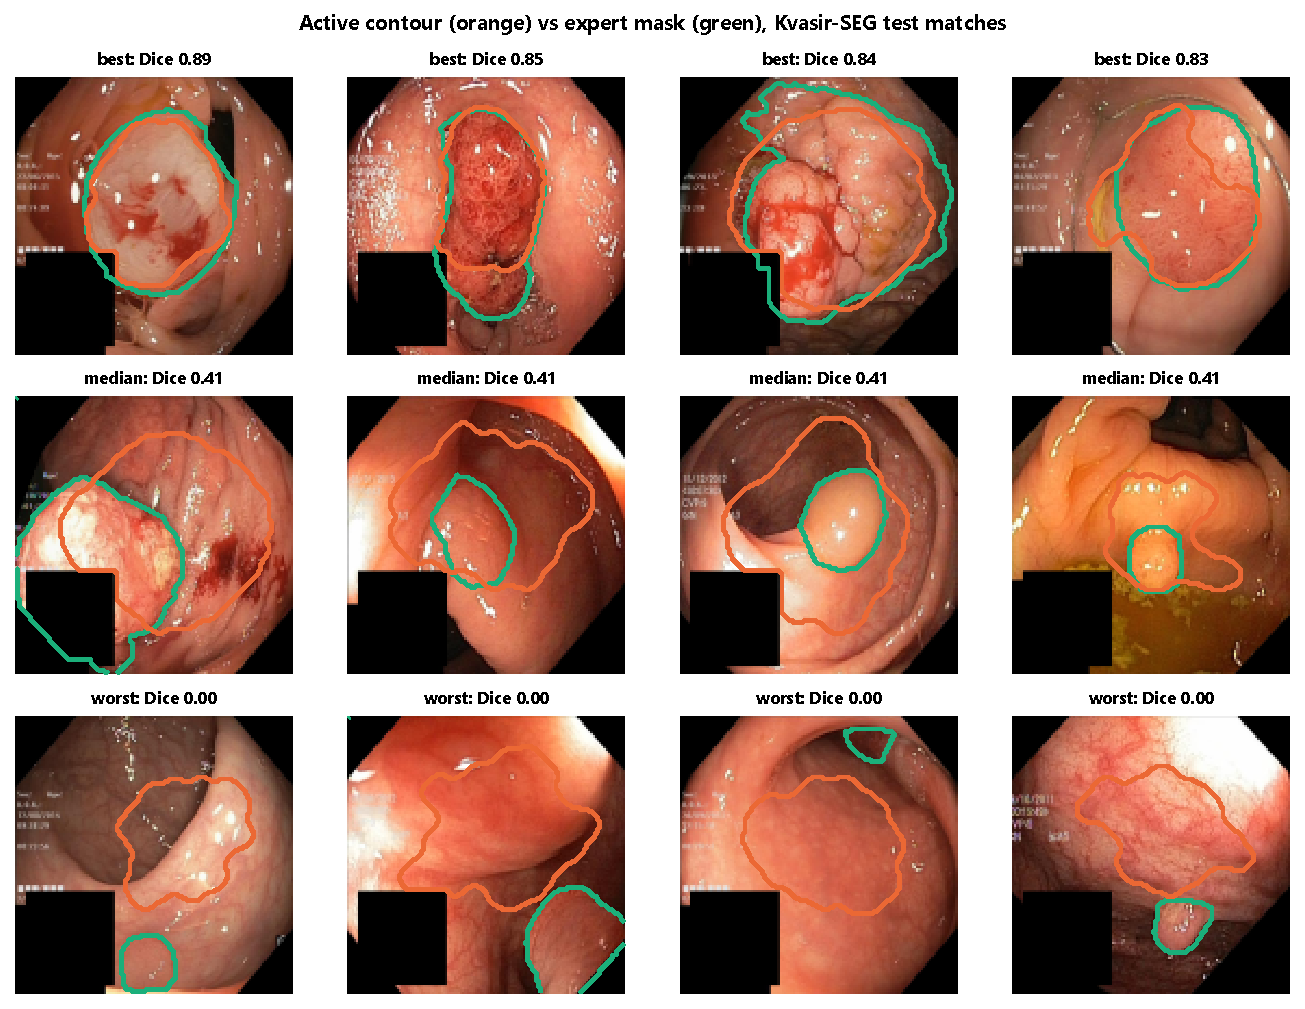
\includegraphics[width=\columnwidth]{ac_gallery.pdf}
\caption{Contour (orange) vs expert mask (green) on Kvasir-SEG test matches: best, median and worst by Dice. Failures are lumen/fold regions and small lesions.}
\label{fig:acgallery}
\end{figure}

\subsection{Classical baselines and feature controls}
Chance is a macro-F1 of \randF{}; the Lab-colour centroid heuristic reaches \heurF{} (polyp AUROC \heurAU{}).
LightGBM on global colour and texture features reaches \lgbGF{}; adding the contour features raises it to \lgbGACF{}.
\emph{However, the controls match or exceed the real contour:} replacing the contour by an image-independent central ellipse gives \lgbGEllF{},
and a contour borrowed from another image gives \lgbGShufF{}. What helps is therefore ``colour and texture inside versus outside a central region'', not the contour itself.
A linear probe on frozen DINOv2 embeddings reaches \dinoProbeF{}, above every hand-crafted pipeline.

\subsection{Deep backbones}
Table~\ref{tab:leaderboard} compares all models under one protocol. Fine-tuned ConvNeXt-T, EfficientNetV2-S, Swin-T and DINOv2 ViT-S/14 lie within about one to two points of each other
(macro-F1 \convnextF{}, \effnetF{}, \swinF{} and \dinoF{}), while the ResNet-50 recipe trails at \resnetF{}. Polyp-vs-rest AUROC is above 0.99 for all fine-tuned networks.
A soft-voting ensemble of the five backbones reaches \ensF{}.
\begin{table*}[t]
\centering
\caption{Held-out test performance (mean$\pm$SD over seeds; deep models $N{=}3$, classical $N{=}5$). Best per column in bold. ECE after temperature scaling.}
\label{tab:leaderboard}
\small
\begin{adjustbox}{max width=\linewidth}\begin{tabular}{lrrrrr}
\toprule
Model & Macro-F1 & Acc. & MCC & Polyp AUROC & ECE \\
\midrule
ResNet-50 & 0.8708{\scriptsize$\pm$0.0043} & 0.8712{\scriptsize$\pm$0.0045} & 0.8530{\scriptsize$\pm$0.0051} & 0.9916{\scriptsize$\pm$0.0017} & 0.0300{\scriptsize$\pm$0.0026} \\
EfficientNetV2-S & 0.9257{\scriptsize$\pm$0.0025} & 0.9258{\scriptsize$\pm$0.0025} & 0.9153{\scriptsize$\pm$0.0029} & \textbf{0.9957{\scriptsize$\pm$0.0004}} & 0.0256{\scriptsize$\pm$0.0035} \\
ConvNeXt-T & 0.9233{\scriptsize$\pm$0.0006} & 0.9235{\scriptsize$\pm$0.0006} & 0.9128{\scriptsize$\pm$0.0007} & 0.9931{\scriptsize$\pm$0.0029} & 0.0353{\scriptsize$\pm$0.0027} \\
Swin-T & 0.9327{\scriptsize$\pm$0.0045} & 0.9327{\scriptsize$\pm$0.0045} & 0.9232{\scriptsize$\pm$0.0051} & 0.9947{\scriptsize$\pm$0.0014} & 0.0306{\scriptsize$\pm$0.0050} \\
DINOv2 ViT-S/14 & \textbf{0.9344{\scriptsize$\pm$0.0058}} & \textbf{0.9343{\scriptsize$\pm$0.0058}} & \textbf{0.9250{\scriptsize$\pm$0.0066}} & 0.9916{\scriptsize$\pm$0.0015} & 0.0242{\scriptsize$\pm$0.0035} \\
ACG-ConvNeXt (full) & 0.9277{\scriptsize$\pm$0.0035} & 0.9279{\scriptsize$\pm$0.0035} & 0.9178{\scriptsize$\pm$0.0040} & 0.9900{\scriptsize$\pm$0.0013} & 0.0325{\scriptsize$\pm$0.0016} \\
ACG-ResNet-50 & 0.8560{\scriptsize$\pm$0.0103} & 0.8565{\scriptsize$\pm$0.0100} & 0.8363{\scriptsize$\pm$0.0114} & 0.9887{\scriptsize$\pm$0.0023} & 0.0353{\scriptsize$\pm$0.0049} \\
LightGBM $\cdot$ global colour/texture & 0.7507{\scriptsize$\pm$0.0037} & 0.7513{\scriptsize$\pm$0.0037} & 0.7160{\scriptsize$\pm$0.0042} & 0.9565{\scriptsize$\pm$0.0003} & 0.1285{\scriptsize$\pm$0.0011} \\
LightGBM $\cdot$ contour features only & 0.8063{\scriptsize$\pm$0.0029} & 0.8073{\scriptsize$\pm$0.0029} & 0.7804{\scriptsize$\pm$0.0033} & 0.9721{\scriptsize$\pm$0.0005} & 0.1450{\scriptsize$\pm$0.0036} \\
LightGBM $\cdot$ global + contour & 0.7954{\scriptsize$\pm$0.0045} & 0.7964{\scriptsize$\pm$0.0045} & 0.7678{\scriptsize$\pm$0.0052} & 0.9716{\scriptsize$\pm$0.0006} & 0.1310{\scriptsize$\pm$0.0056} \\
Logistic reg. $\cdot$ global + contour & 0.7763 & 0.7773 & 0.7458 & 0.9712{\scriptsize$\pm$0.0000} & 0.0308{\scriptsize$\pm$0.0000} \\
LightGBM $\cdot$ global + central-ellipse features (control) & 0.8003{\scriptsize$\pm$0.0028} & 0.8005{\scriptsize$\pm$0.0028} & 0.7721{\scriptsize$\pm$0.0032} & 0.9788{\scriptsize$\pm$0.0002} & 0.1303{\scriptsize$\pm$0.0027} \\
LightGBM $\cdot$ global + shuffled-contour features (control) & 0.7840{\scriptsize$\pm$0.0013} & 0.7847{\scriptsize$\pm$0.0014} & 0.7542{\scriptsize$\pm$0.0016} & 0.9695{\scriptsize$\pm$0.0004} & 0.1338{\scriptsize$\pm$0.0008} \\
RBF-SVM $\cdot$ global + contour & 0.7900 & 0.7905 & 0.7609 & 0.9749{\scriptsize$\pm$0.0000} & \textbf{0.0219} \\
Random forest $\cdot$ global + contour & 0.7658{\scriptsize$\pm$0.0044} & 0.7666{\scriptsize$\pm$0.0044} & 0.7338{\scriptsize$\pm$0.0051} & 0.9624{\scriptsize$\pm$0.0004} & 0.1079{\scriptsize$\pm$0.0044} \\
XGBoost $\cdot$ global + contour & 0.7947{\scriptsize$\pm$0.0045} & 0.7955{\scriptsize$\pm$0.0044} & 0.7667{\scriptsize$\pm$0.0051} & 0.9735{\scriptsize$\pm$0.0011} & 0.1179{\scriptsize$\pm$0.0054} \\
Linear probe $\cdot$ frozen DINOv2 & 0.8889{\scriptsize$\pm$0.0000} & 0.8890 & 0.8732 & 0.9951{\scriptsize$\pm$0.0000} & 0.0354 \\
Random guess & 0.1311 & 0.1311 & 0.0070 & 0.4947 & 0.2116 \\
Class prior (majority) & 0.0279 & 0.1255 & 0.0000 & 0.4917 & 0.0000 \\
Heuristic $\cdot$ nearest Lab-colour centroid & 0.4762 & 0.4793 & 0.4066 & 0.8372 & 0.2669 \\
\bottomrule
\end{tabular}\end{adjustbox}
\end{table*}

\subsection{Does contour guidance help? (RQ1, RQ2)}
Table~\ref{tab:ablation} and Fig.~\ref{fig:forest} give the ablation on ConvNeXt-T. Plain ConvNeXt-T scores \plainF{}$\pm$\plainFSD{}. The full ACG model scores \acgF{}$\pm$\acgFSD{}
($\Delta=$ \acgDelta{}, 95\,\% CI \acgDeltaLo{} to \acgDeltaHi{}, Holm-adjusted $p=$ \acgPHolm{}).
\textbf{The difference is not statistically supported}, and neither are the shuffled-image control (\shufDelta{}) and the ellipse control (\ellDelta{}): all three overlap.
Non-contour global features alone give \gfeatDelta{}, the largest and only nominally significant bootstrap difference, which does not survive Holm correction (adjusted $p=$ \gfeatPHolm{}).
Seed-level paired $t$-tests with $N{=}3$ are fragile (the plain model's seed SD is only \plainFSD{}, which inflates standardised effect sizes) and are therefore reported in the repository but not relied on.
Generality: ACG on ResNet-50 scores \resacgF{}\,$\pm$\,\resacgFSD{} against \resnetF{} for plain ResNet-50.
\begin{table*}[t]
\centering
\caption{Ablation on ConvNeXt-T ($N{=}3$ seeds). $\Delta$: seed-averaged macro-F1 difference to the plain baseline with 95\,\% paired-bootstrap interval over test images; $p$: Holm-adjusted bootstrap p-value.}
\label{tab:ablation}
\small
\begin{adjustbox}{max width=\linewidth}\begin{tabular}{lrrrl r}
\toprule
Variant & Macro-F1 & Acc. & Polyp AUROC & $\Delta$ [95\,\% CI] & $p_\mathrm{Holm}$ \\
\midrule
ConvNeXt-T (plain) & 0.9233{\scriptsize$\pm$0.0006} & 0.9235 & 0.9931 & +0.0000 -- & -- \\
+ global hand-crafted features & 0.9295{\scriptsize$\pm$0.0035} & 0.9295 & 0.9927 & +0.0062 [+0.0013, +0.0111] & 0.072 \\
+ contour pooling & 0.9264{\scriptsize$\pm$0.0037} & 0.9264 & 0.9934 & +0.0031 [-0.0015, +0.0075] & 0.380 \\
+ contour features & 0.9288{\scriptsize$\pm$0.0003} & 0.9289 & 0.9932 & +0.0055 [+0.0004, +0.0106] & 0.180 \\
ACG-ConvNeXt (full) & 0.9277{\scriptsize$\pm$0.0035} & 0.9279 & 0.9900 & +0.0045 [-0.0004, +0.0091] & 0.296 \\
full, shuffled contours (control) & 0.9275{\scriptsize$\pm$0.0015} & 0.9276 & 0.9912 & +0.0043 [-0.0010, +0.0093] & 0.354 \\
full, central ellipse (control) & 0.9267{\scriptsize$\pm$0.0067} & 0.9268 & 0.9908 & +0.0035 [-0.0017, +0.0085] & 0.380 \\
\bottomrule
\end{tabular}\end{adjustbox}
\end{table*}
\begin{figure}[t]
\centering
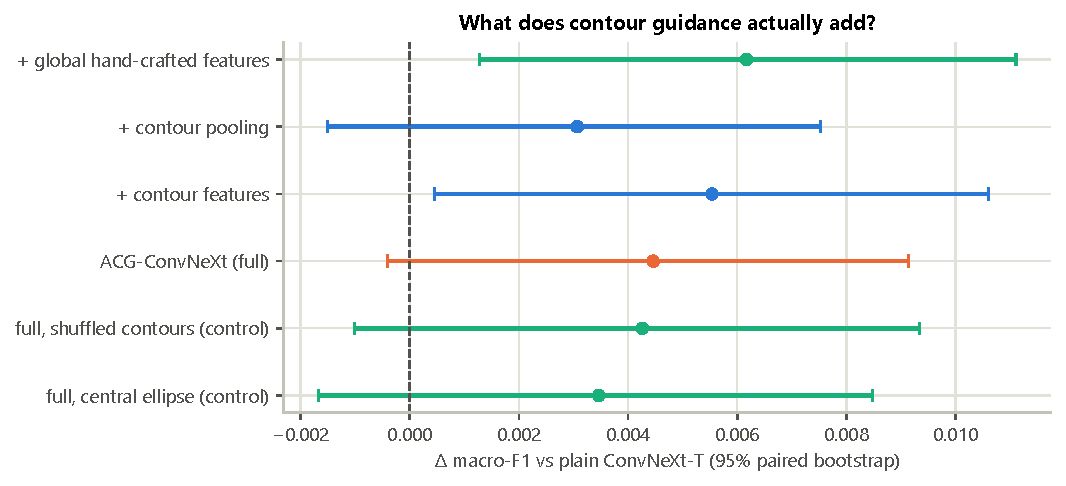
\includegraphics[width=\columnwidth]{ablation_forest.pdf}
\caption{Difference in macro-F1 to plain ConvNeXt-T with 95\,\% paired-bootstrap intervals (unadjusted). The full model and both image-independent controls are indistinguishable.}
\label{fig:forest}
\end{figure}

\subsection{Shortcuts and leakage (RQ3)}
Despite the strong metadata shortcuts (Section~\ref{sec:data}), a ConvNeXt-T trained on \emph{naive} full frames (no crop, no artefact mask) reaches \naiveF{}\,$\pm$\,\naiveFSD{},
statistically equal to the canonical \plainF{}: the shortcuts separate upper-GI from colon, which pixels already do, while the remaining errors are within-region pairs where neither shortcut carries information.
Training and testing on a \emph{random} split with the same sizes gives \randsplitF{}\,$\pm$\,\randsplitFSD{} (different test images, so not paired), consistent with the modest \randLeakPct{} near-duplicate overlap measured in the audit.

\subsection{Calibration and conformal prediction (RQ5)}
Temperature scaling reduces ECE from \eceRaw{} to \eceCal{}. Validation-calibrated conformal sets reach only \confCovVal{} coverage at a nominal 95\,\%,
because the validation split was reused for early stopping, temperature and threshold and is therefore optimistic. Calibrating on a random half of the test \emph{scene groups} and evaluating on the other half
(200 repeats) restores coverage: \confCov{}\,$\pm$\,\confCovSD{}, mean set size \confSize{}, \confSingle{} singleton sets (Fig.~\ref{fig:cal}).
For polyp-vs-rest, at a miss cost five times a false alarm, the 0.5 threshold has expected cost \costHalf{} per image against \costYouden{} for the validation-Youden threshold and \costOpt{} for the validation cost-optimal threshold:
thresholds tuned on the optimistic validation split did not beat the default.
\begin{figure}[t]
\centering
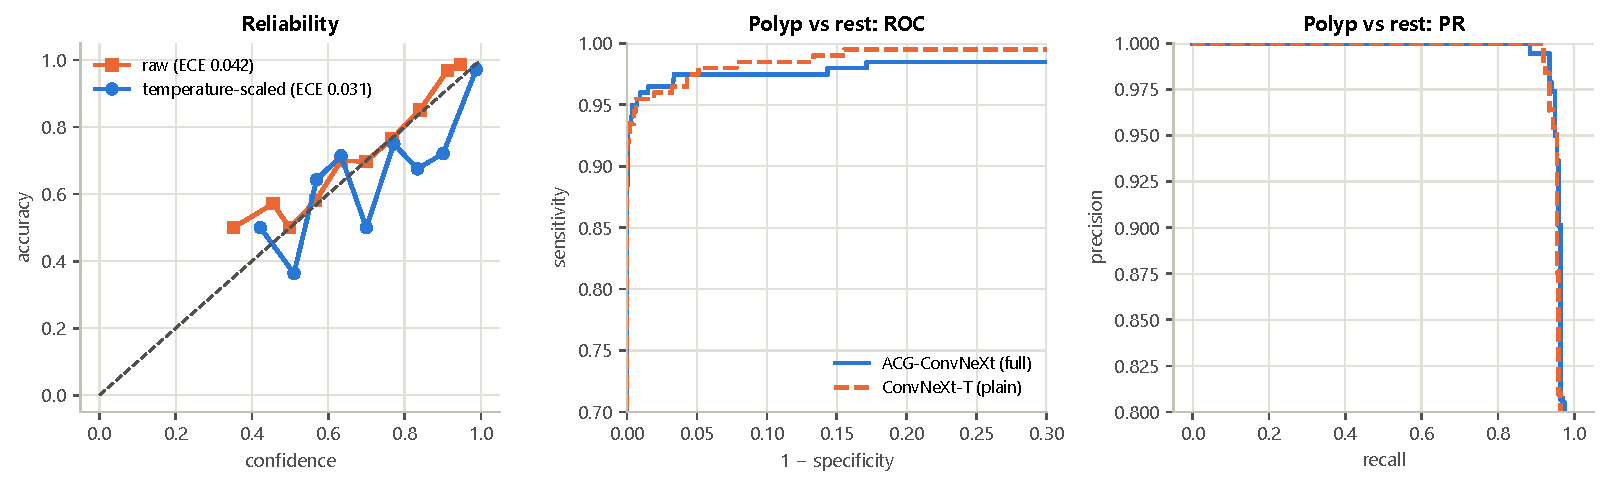
\includegraphics[width=\columnwidth]{calibration_roc_pr.pdf}
\caption{Reliability before/after temperature scaling, and polyp-vs-rest ROC and PR curves (seed 0).}
\label{fig:cal}
\end{figure}

\subsection{Error analysis}
Of \nErrors{} test errors (\errRate{}), \errPairs{} fall into two confusable pairs (esophagitis$\leftrightarrow$z-line and dyed-lifted$\leftrightarrow$dyed-resection-margins; Fig.~\ref{fig:conf}).
\errFlagged{} of the errors involve images flagged by confident learning, against \corrFlagged{} of correct predictions, so a large share of the residual error is label ambiguity rather than model failure.
We inspected the 36 most confident errors (a visual judgement by a non-clinician, not an adjudication): 17 are esophagitis$\leftrightarrow$z-line, 7 are dyed-lifted$\leftrightarrow$resection-margin, 7 are ``polyp'' frames with no distinct visible lesion (the clinically important group, only 2 of which are flagged), and 5 are other colitis/cecum mixes; 26 of the 36 are flagged.
The most confident errors (Fig.~\ref{fig:err}) show craters with dye that are plausible for either dyed class, homogeneous mucosa labelled ``polyp'' with no visible lesion, and z-line frames with inflammation.
Accuracy is \accColonScope{} on colon-scope (720$\times$576) frames and \accUpperScope{} on larger-format upper-GI frames; the worst class accuracy is \worstClassAcc{}.
\begin{figure}[t]
\centering
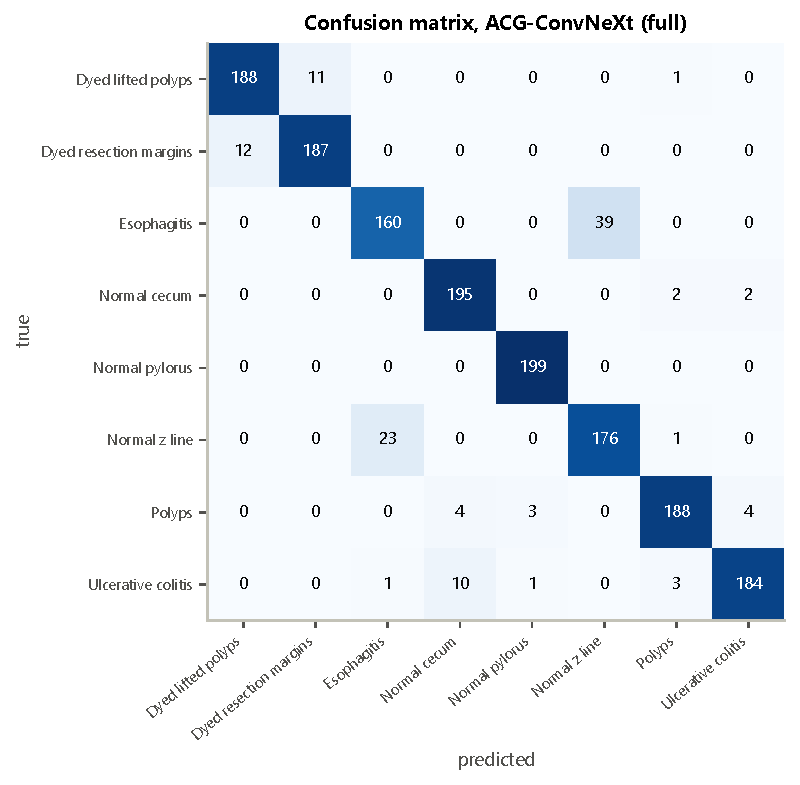
\includegraphics[width=0.85\columnwidth]{confusion_matrix.pdf}
\caption{Confusion matrix of the seed-ensembled ACG-ConvNeXt on the test split.}
\label{fig:conf}
\end{figure}
\begin{figure*}[t]
\centering
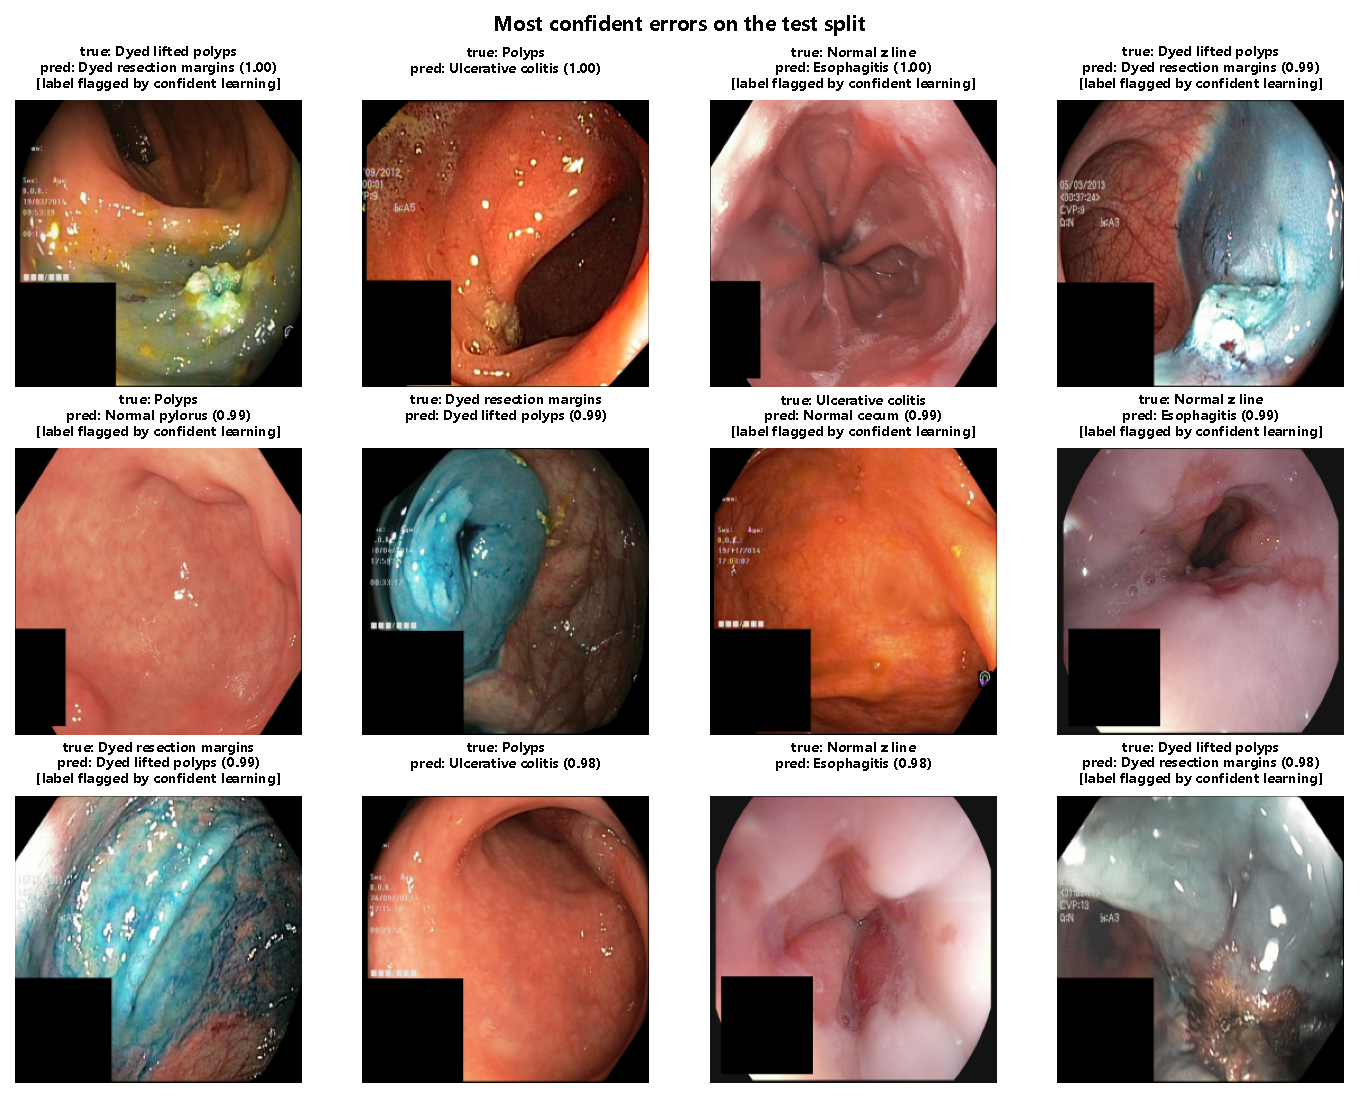
\includegraphics[width=0.8\textwidth]{error_gallery.pdf}
\caption{The twelve most confident errors, with confident-learning flags.}
\label{fig:err}
\end{figure*}

\subsection{Data efficiency, robustness and interpretability (RQ4)}
\paragraph{Data efficiency (RQ4).}
Training on 10\,\%, 25\,\%, 50\,\% and 100\,\% of the training split gives macro-F1 \lcNoneTen{}, \lcNoneTwentyFive{}, \lcNoneFifty{}, \lcNoneFull{} for the plain model and
\lcAcgTen{}, \lcAcgTwentyFive{}, \lcAcgFifty{}, \lcAcgFull{} for ACG-ConvNeXt (Fig.~\ref{fig:lc}). The curves overlap: guidance does not help more when data are scarce.
\begin{figure}[t]
\centering
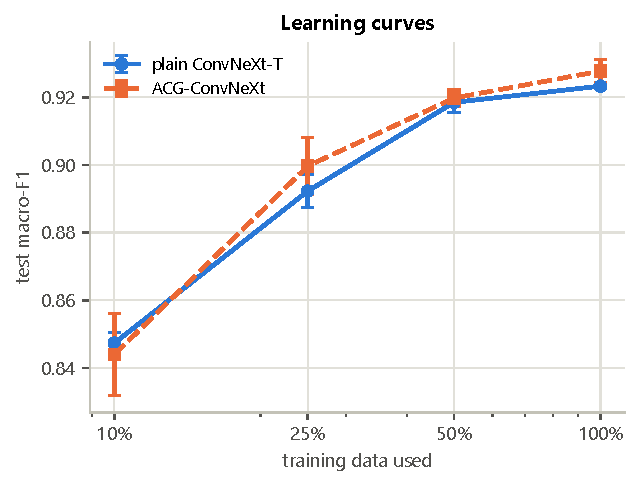
\includegraphics[width=0.8\columnwidth]{learning_curves.pdf}
\caption{Learning curves (mean $\pm$ SD over 3 seeds).}
\label{fig:lc}
\end{figure}

\paragraph{Learning-rate sensitivity.}
Deep hyper-parameters were not tuned per variant. For seed 0, the plain model scores \lrNoneHalf{}, \lrNoneDef{} and \lrNoneDouble{} at half, default and double learning rate, and the guided model \lrAcgHalf{}, \lrAcgDef{} and \lrAcgDouble{}:
changing the learning rate moves macro-F1 by as much as any ablation effect, and the default rate was evidently not optimal for the plain model.
The guided model's seed-0 score at the doubled rate looked like a clear gain, but that rate was singled out after seeing test results, so we replicated it as an exploratory, post hoc check with three seeds per variant:
plain \lrTwoPlain{}\,$\pm$\,\lrTwoPlainSD{}, guided \lrTwoAcg{}\,$\pm$\,\lrTwoAcgSD{} ($\Delta=$ \lrTwoDelta{}, 95\,\% CI \lrTwoLo{} to \lrTwoHi{}, unadjusted bootstrap $p=$ \lrTwoP{}).
Both variants improve over the default rate and the gap between them is not distinguishable from zero, so the null conclusion holds at the better learning rate as well. A fully fair comparison would tune every variant on validation data, which we did not do.

\paragraph{Robustness.}
On \robN{} stratified test frames, JPEG compression at quality 50 lowers accuracy from \robPlainClean{} to \robPlainJpegFifty{} for the plain model, but only from \robAcgClean{} to \robAcgJpegFifty{} for the guided model (Fig.~\ref{fig:rob}).
At quality 10 the figures are \robPlainJpegTen{} against \robAcgJpegTen{}, and under Gaussian blur with $\sigma=3$\,px \robPlainBlurThree{} against \robAcgBlurThree{}.
\emph{The controls reproduce this advantage:} shuffled-image contours give \robShufJpegFifty{} and the central ellipse \robEllJpegFifty{} at quality 50, and global features alone give \robGfeatJpegFifty{}.
Robustness therefore comes from supplying colour and texture statistics computed on the pixels, not from the contour's alignment with the lesion.
\begin{figure*}[t]
\centering
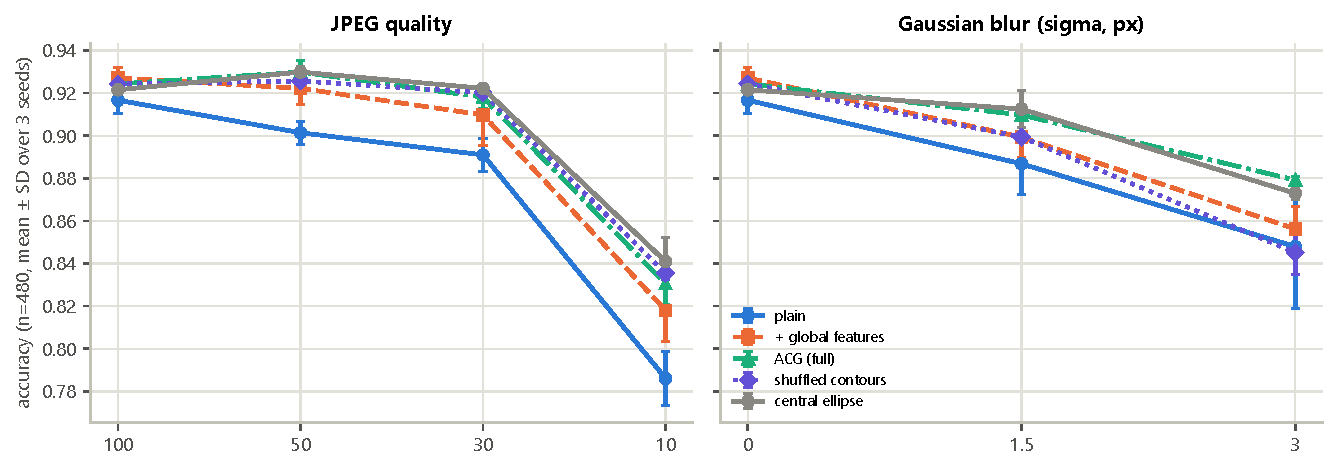
\includegraphics[width=0.7\textwidth]{robustness_multiseed.pdf}
\caption{Accuracy under JPEG compression and Gaussian blur (mean $\pm$ SD over 3 seeds, 480 test frames; contours and features recomputed on the degraded pixels).}
\label{fig:rob}
\end{figure*}

\paragraph{Interpretability.}
\emph{Grad-CAM against expert masks.} Using the polyp-class Grad-CAM on the 176 Kvasir-SEG test-split polyps, the CAM maximum lies inside the expert mask for \plainPoint{} of frames for the plain model and \acgPoint{} for the guided model;
the top-20\,\% CAM pixels overlap the mask with IoU \plainCamIoU{} and \acgCamIoU{}. The CAM maximum falls inside the active contour for \plainCamInAC{} and \acgCamInAC{} of frames.
With $n=176$ these differences are within sampling noise: the guided network does not attend to lesions more accurately than the plain one.
\emph{TreeSHAP} on LightGBM with global and contour features attributes \shapRegion{} of the total importance to inside/outside colour and texture (region) features and \shapGlobal{} to global features, but only \shapShape{} to contour shape and \shapBoundary{} to boundary features:
the geometry of the contour carries little information.
\emph{Layer-wise linear probes} on ConvNeXt-T stages give macro-F1 \lwPreOne{} (pretrained) and \lwFtOne{} (fine-tuned) at stage~1, \lwPreThree{} and \lwFtThree{} at stage~3, and \lwPreFour{} and \lwFtFour{} at stage~4:
fine-tuning mostly reshapes the last two stages.


